% ====================================================================
%+
% SECTION:
%    gw.tex
%
% CHAPTER:
%    transients.tex
%
% ELEVATOR PITCH:
%-
% ====================================================================

\section{Gravitational Wave Sources}
\def\secname{\chpname:gw}\label{sec:\secname}

\credit{raffaellamargutti},
\credit{Doctor},
\credit{Fong},
\credit{Haiman},
\credit{Kalogera},
\credit{Trimble},
\credit{Zauderer}

The first detection of Gravitational Waves (GW) by the advanced
LIGO/Virgo collaboration \citep{Abbott16, Abbott09, Acernese08} has
recently opened a new window of exploration into our Universe. The
amount of information that can be revealed by the properties of the GW
emission is immense and holds promises for revolutionary insights,
including accurate masses and spins of neutron stars and black holes,
tests of General Relativity and an accurate census of the neutron star
(NS) and black hole (BH) populations that might challenge our current
understanding of massive stellar evolution. However, GW events are
poorly localized (10-100 deg$^2$ at the time of LSST operations). The
identification of EM counterparts would provide precise localization and
distance measurements, in addition to the necessary astrophysical
context (e.g. host galaxy properties, connection to specific stellar
populations) to fully exploit the revolutionary power of this new GW
era.

% --------------------------------------------------------------------

\subsection{Target measurements and discoveries}
\label{sec:\secname:targets}

The first GW event was found to be associated with the merger of two
black holes \citep{Abbott16,Abbott16b}. Although no EM counterpart was
expected to accompany a black-hole black-hole (BBH) merger, it seems now
possible that even BBH mergers  might produce short GRB-like EM emission
\citep{Connaughton16,Loeb16,Zhang16,Perna16,Stone16}. Indeed, in
analogy with supermassive BH mergers, shocks might develop in the
just-formed circumbinary accretion disk (if a disk forms), which can
produce a bright afterglow following the BBH merger (e.g.
\citealt{Lippai08,Corrales10,Schnittman13}). Albeit speculative in
nature, it is advisable to keep an open mind about the possibility of EM
counterparts to BBH mergers.

The most promising and better understood EM counterparts to GW events
are ``kilonovae" \citep{Li98,Metzger10,Metzger12,Kasen13,Barnes13}.
Kilonovae are short-lived (typical time scale of one week), apparently
faint ($z\sim21$ mag at peak at 120 Mpc), red ($i-z\approx1$ mag),
isotropic transients (\autoref{Fig:kilonova}) due to the radioactive
decay of r-process elements synthesized in the merger ejecta of a NS-NS
or NS-BH system. These merging systems are the favored progenitors of
short GRBs. Indeed, a signature consistent with kilonova emission has been
recently found following the short GRB\,130603B
\citep{Berger13,Tanvir13}. The key piece of information that enabled the
discovery of kilonova-like emission associated with  this short GRB was
its sub-arcsecond localization enabled by the detection of the optical
afterglow, which allowed for an effective kilonova search with the
Hubble Space Telescope (\autoref{Fig:kilonova}). In contrast, the
typical localization region of GW events in the LSST era is expected to
be of the order of a few tens of square degrees \citep{aaa+13}. It is
thus clear that the major challenges faced by the optical follow-up of
GW events is represented by the combination of poor localizations with
faint and fast evolving red electromagnetic counterparts.

The detection of an optical counterpart in conjunction with a GW event
will significantly leverage the GW signal. LSST, with its the wide FOV,
wavelength coverage and exquisite sensitivity is uniquely poised to
identify and characterize counterparts to GW events.

\begin{figure}
\vskip -0.0 true cm
\centering
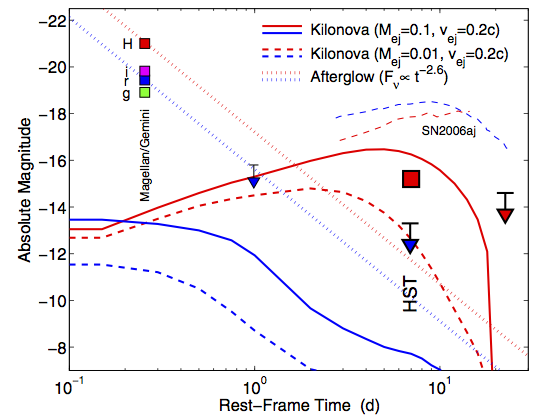
\includegraphics[scale=0.85]{figs/transients/kilonovaBerger.png}
\caption{Kilonova signature in the short GRB\,130603B as revealed by the
Hubble Space Telescope (HST). The Magellan and Gemini telescopes sampled
the optical afterglow of the GRB (dotted lines). The kilonova light
starts to dominate the emission in the H band around a few days after
the merger. Thick and dashed lines: theoretical kilonova models from
\citet{Barnes13} showing that kilonovae are fast-evolving, faint and red
transients. The light-curve of the SN\,2006aj associated with the long
GRB\,060218  is also shown for comparison. From \citet{Berger13}.}
\label{Fig:kilonova}
\end{figure}


% --------------------------------------------------------------------

\subsection{OpSim Analysis and Discussion}
\label{sec:\secname:analysis}

Effective follow up of GW triggers relies on the capability to sample a
relatively large portion of the sky, repeatedly, over a time scale $<1$
week, with different filters \citep{Cowperthwaite15}. In the optical
band, the kilonova signature is expected to be more prominent in the
$i$, $z$  and $y$ filters, which we identify as the most promising
filters for the kilonova search. We emphasize however that another set
of contemporaneous observations in  a ``bluer" filter is necessary to
acquire color information and distinguish kilonovae from other
fast-evolving transients.

We use the median inter-night gap  for visits in the same filter derived
from the candidate Baseline Cadence \opsimdbref{db:baseCadence} to show that,
in the absence of a Target of Opportunity (ToO) capability, it is
\emph{not} possible for LSST  to play a major role in the identification
of EM counterparts of GW triggers.

To identify kilonova candidates we need at least 2 observations acquired
within $\sim 1$ week  of the GW event \citep{Cowperthwaite15}. Using the
inter-night gap distribution for visits in the $y$ filter (which is the
most promising filter for a kilonova search), the area of the sky
covered with cadence  $\Delta t<7$ days at any given time, is
$A_{sky}\sim 3000$ deg$^2$ (including deep drilling fields).  This is
the area that can be searched for fast evolving transients.  Two
important considerations follow:

\begin{itemize}
\item[(1)] $A_{sky}$ only covers $P\sim7$\% of the sky. The  probability
that the \emph{entire} GW localization region is contained, by chance,
within $A_{sky}$ is thus very small.
\item[(2)] Even if LSST is able to cover a meaningful portion of the GW
region, we would still not have color information, and we would thus be
unable to filter out contaminating transients.
\end{itemize}

\textit{We conclude that relying on the serendipitous alignment of the
LSST fields with the GW localization map is not an effective strategy to
follow up GW triggers and identify their EM counterparts. We thus
strongly recommend a ToO capability as part of the baseline LSST
operations strategy.}

Ideally, the ToO capability will allow for imaging of the GW
localization map at least twice over $\Delta t\lesssim$1 week with a
``red" filter ($i$, $z$  or $y$),  and  will include the possibility to
designate a desired set of filters to obtain color information. By the
time of LSST operation the typical size of the GW localization region is
expected to be 10-100 deg$^2$, which would require a small number of
LSST re-pointings. We thus do \emph{not} anticipate a significantly
disruptive impact on other LSST campaigns (especially if only the GW
triggers with the best localizations in the southern sky are selected
for LSST ToOs).

\textit{At the price of re-shuffling a reasonably small number of
fields, \textbf{if} equipped with ToO capabilities, LSST can be the
premier player in the era of EM follow up to GW sources.}

% ====================================================================
%
% \subsection{Conclusions}
%
% Here we answer the ten questions posed in
% \autoref{sec:intro:evaluation:caseConclusions}:
%
% \begin{description}
%
% \item[Q1:] {\it Does the science case place any constraints on the
% tradeoff between the sky coverage and coadded depth? For example, should
% the sky coverage be maximized (to $\sim$30,000 deg$^2$, as e.g., in
% Pan-STARRS) or the number of detected galaxies (the current baseline 
% of 18,000 deg$^2$)?}
%
% \item[A1:] ...
%
% \item[Q2:] {\it Does the science case place any constraints on the
% tradeoff between uniformity of sampling and frequency of  sampling? For
% example, a rolling cadence can provide enhanced sample rates over a part
% of the survey or the entire survey for a designated time at the cost of
% reduced sample rate the rest of the time (while maintaining the nominal
% total visit counts).}
%
% \item[A2:] ...
%
% \item[Q3:] {\it Does the science case place any constraints on the
% tradeoff between the single-visit depth and the number of visits
% (especially in the $u$-band where longer exposures would minimize the
% impact of the readout noise)?}
%
% \item[A3:] ...
%
% \item[Q4:] {\it Does the science case place any constraints on the
% Galactic plane coverage (spatial coverage, temporal sampling, visits per
% band)?}
%
% \item[A4:] ...
%
% \item[Q5:] {\it Does the science case place any constraints on the
% fraction of observing time allocated to each band?}
%
% \item[A5:] ...
%
% \item[Q6:] {\it Does the science case place any constraints on the
% cadence for deep drilling fields?}
%
% \item[A6:] ...
%
% \item[Q7:] {\it Assuming two visits per night, would the science case
% benefit if they are obtained in the same band or not?}
%
% \item[A7:] ...
%
% \item[Q8:] {\it Will the case science benefit from a special cadence
% prescription during commissioning or early in the survey, such as:
% acquiring a full 10-year count of visits for a small area (either in all
% the bands or in a  selected set); a greatly enhanced cadence for a small
% area?}
%
% \item[A8:] ...
%
% \item[Q9:] {\it Does the science case place any constraints on the
% sampling of observing conditions (e.g., seeing, dark sky, airmass),
% possibly as a function of band, etc.?}
%
% \item[A9:] ...
%
% \item[Q10:] {\it Does the case have science drivers that would require
% real-time exposure time optimization to obtain nearly constant
% single-visit limiting depth?}
%
% \item[A10:] ...
%
% \end{description}

% ====================================================================

\navigationbar
